\documentclass[20pt,a4paper]{report}
\usepackage[T2A,T1]{fontenc}
\usepackage[utf8]{inputenc}
\usepackage{blindtext}
\usepackage[russian]{babel}
\usepackage{mwe}
\usepackage{graphbox}
\usepackage[document]{ragged2e}
\usepackage[margin=50pt]{geometry}
\usepackage{longtable}
\usepackage{fontspec}
\usepackage{float}
\usepackage{titlesec}
\usepackage{setspace}
\usepackage{minted}

\usepackage{hyperref}
\hypersetup{
    colorlinks,
    citecolor=black,
    filecolor=black,
    linkcolor=black,
    urlcolor=black
}

\setstretch{1.5}
\graphicspath{{./images/}}
\setmainfont{LiberationSerif}
\setmonofont{Hack}
\titleformat{\chapter}{\normalfont\LARGE\bfseries}{\thechapter}{1em}{}
\titleclass{\chapter}{straight}
\titlespacing{\chapter}{0pt}{0pt}{5pt}[25pt]


\begin{document}
	\begin{titlepage}
		\begin{minipage}{0.3\textwidth}
		
\includegraphics[scale=0.03]{logo.png}	
		\end{minipage}
		\begin{minipage}{0.6\textwidth}\centering
			\textbf{
				Министерство науки и высшего образования Российской Федерации
				Федеральное государственное бюджетное образовательное 
				учреждение высшего образования
				«Московский государственный технический университет
				имени Н.Э. Баумана (национальный исследовательский университет)»
				(МГТУ им. Н.Э. Баумана)
			}	
		\end{minipage}
	
		\vspace{5cm}
		\centering
		\Large
		\textbf{
			Лабораторная работа №6 \\
			по курсу «Разработка интернет-приложений» \\
		}

		\vspace{6cm}
		\begin{flushright}
			Выполнил \\ 
			студент группы ИУ5-54Б \\ 
			Сысойкин Е.М. 
		\end{flushright}
		\vspace{5cm}
		Москва, 2020
	\end{titlepage}

	\chapter{Описание задания}
		\large
		\qquad Разработать HTML-форму, содержащую следующие элементы: \\
		\begin{enumerate}
			\item Текстовое однострочное поле ввода.
			\item Набор элементов checkbox.
			\item Набор радиокнопок.
			\item Текстовое поле ввода из нескольких строк.
			\item Список.
			\item Выпадающий список.
			\item Список на основе текстового поля.
			\item Кнопку с изображением.
			\item Кнопку отправки формы.
		\end{enumerate}

	\chapter{Текст программы}
		\qquad \textbf{index.html} \\
		\small
		\inputminted[tabsize=4, linenos]{html}{index.html}
		\large
		
	\chapter{Экранные формы}
		\begin{figure}[H]
			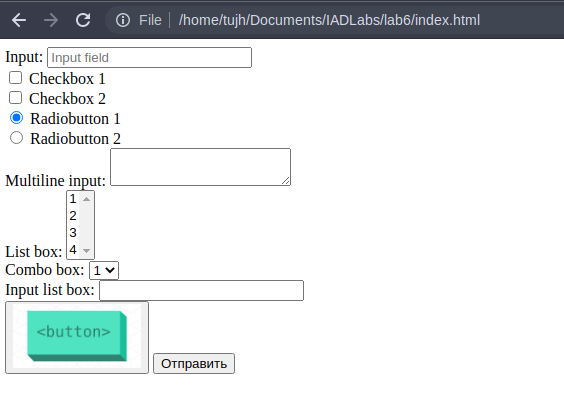
\includegraphics[width=\textwidth]{1.png}
		\end{figure}

\end{document}

